% Document layout
\documentclass[a4paper,11pt]{article}
\usepackage[a4paper, inner=2.5cm , outer=2.5cm, top=2cm, bottom=2cm]{geometry}
\usepackage[usenames,dvipsnames]{color}
% Referencing & fonts
\usepackage[sort&compress]{natbib}
\setlength{\bibsep}{0.0pt}
\usepackage[font=small,labelfont=bf]{caption}
\usepackage[OT2,T1]{fontenc}
% Set formats for each heading level
\usepackage{sectsty}
\allsectionsfont{\usefont{OT1}{phv}{bc}{n}\selectfont}
\sectionfont{\color{MidnightBlue}} % sets colour of sections
\subsectionfont{\color{MidnightBlue}}  % sets colour of subsections
\subsubsectionfont{\color{MidnightBlue}}  % sets colour of subsections
% Other shit
\usepackage{algorithm}
\usepackage{amsfonts}
\usepackage{amsmath}
\usepackage{amssymb}
\usepackage{bbm}
\usepackage{booktabs}
\usepackage{epsfig}
\usepackage{float}
\usepackage[font=normalsize]{caption}
\usepackage{graphicx}
\usepackage{hyperref}
\usepackage{lineno}
\usepackage{mathtools}
\usepackage{sidecap}
\usepackage{sectsty}
\usepackage{verbatim}
\usepackage{wrapfig}
\usepackage{xcolor}
% Declarations
\DeclarePairedDelimiter\floor{\lfloor}{\rfloor}
\DeclareSymbolFont{cyrletters}{OT2}{wncyr}{m}{n}
\DeclareMathSymbol{\Sha}{\mathalpha}{cyrletters}{"58}
\DeclareMathSymbol{\sha}{\mathalpha}{cyrletters}{"57}
% Defined commands
 \newcommand{\prgname}[1]{\textcolor{NavyBlue}{\texttt{#1}}}
 \newcommand{\linkfont}[1]{\textcolor{BurntOrange}{\textbf{#1}}}
\newcommand{\shellcmd}[1]{\\\indent\indent\texttt{\$ #1}}
\newcommand{\shellctd}[1]{\\\indent\indent\texttt{#1}}
\newcommand{\ra}[1]{\renewcommand{\arraystretch}{#1}}
\begin{document}
\begin{figure}
\centering
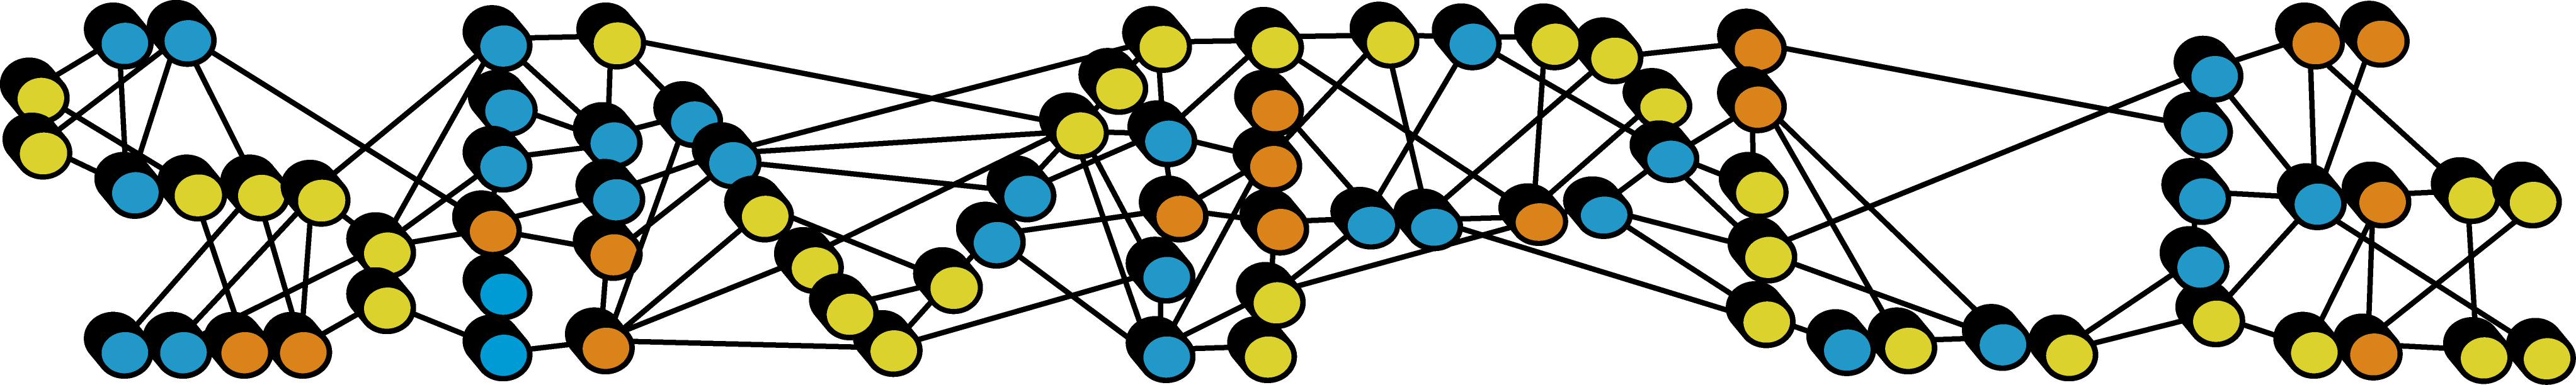
\includegraphics[keepaspectratio=true,scale=0.6]{./SIMPLE_logo/rawlogo}
%\caption{}
\end{figure}

\title{\prgname{SIMPLE Workshop 2017}}
\author{Dominika Elmlund, Hans Elmlund}
\maketitle

\vspace{1em}
\begin{minipage}[ht]{0.48\textwidth}
\textbf{Contributors:}\\
cyril.reboul@monash.edu\\
dominika.elmlund@monash.edu\\
hans.elmlund@monash.edu\\
\textbf{Adress:}\\
Dept. Biochemistry and Molecular Biology\\
School of Biomedical Sciences\\
Monash University, Bldg. 77\\
Clayton, VIC, Australia, 3800\\
\textbf{Webpage:}\\
www.simplecryoem.com\\
\end{minipage}
\vspace{20pt}

\section{What Will Be Covered}
This part of the workshop will cover 
\begin{enumerate}
\item DDD (Direct Detector Device) movie pre-processing
\item 2D analysis with PRIME2D
\item \textit{ab initio} 3D reconstruction from class averages using PRIME3D
\end{enumerate}
with the SIMPLE program package. We will use the latest unreleased version of SIMPLE, available to the workshop participants for downloading and beta-testing on the SIMPLE homepage \url{http://simplecryoem.com/beta.html}.

\section{DDD Movie Pre-Processing}
During image acquisition, beam induced motion, charging and stage drift introduce blurring in the integrated movies. The individual frames need to be aligned with respect to one another in order to restore high-resolution information. Because of radiation damage, the electron dose is kept low during image acquisition, resulting in a very low signal-to-noise ratio (SNR) of the individual movie frames. Until recently, our understanding of damage processes in cryo-EM was based primarily on results obtained with 2D protein crystals (REFS 44,45 REVIEW). The use of 2D crystals provides direct means for assessing the degree of damage by looking at the rate by which high-resolution diffraction spots are fading as a function of the accumulative electron dose. The disadvantage here is that it is impossible to separate spot fading due to loss of crystalline order from intrinsic molecular damage. Images of single rotavirus VP6 particles recorded with a total exposure of 100 electrons/�2 indicated that single-particles are more robust to damage at low and intermediate resolution than previously thought (REF 46 REVIEW). In the same study, a dose-weighting scheme was introduced that maximizes the SNR of the integrated movie in a dose-dependent manner. This dose-weighting strategy has been adopted by most software packages and proven to be a powerful addition to the ever-growing set of single-particle analysis tools.

SIMPLE implements a program called \prgname{unblur\_movies} for simultaneous motion-correction and dose-weighting, with the objective of maximising the SNR of the integrated movie in a motion- and dose-dependent manner. Input is a text file \texttt{filetab}, simply listing the individual movies in \texttt{*.mrc} format, the pixel-to-pixel (or sampling) distance \texttt{smpd} (in A), the number of CPU threads to use \texttt{nthr}, the body of the outputted files \texttt{fbody}, the exposure time of the movie \texttt{exp\_time} (in s), the dose-rate at which the movie was acquired \texttt{dose\_rate} (in e/A2/s) and the acceleration voltage of the electron microscope \texttt{kv} (in kV), in addition to a number of other optional parameters that we will not be concerned with here. If we execute \texttt{simple\_exec prg=unblur\_movies} in the prompt, we obtain brief instructions for how to run the program:
\begin{verbatim}
@!#> simple_exec prg=unblur_movies
USAGE:
bash-3.2$ simple_exec prg=simple_program key1=val1 key2=val2 ...

REQUIRED
filetab = list of files(*.txt/*.asc)
smpd    = sampling distance, same as EMANs apix(in A)

OPTIONAL
nthr      = nr of OpenMP threads{1}
fbody     = file body
lpstart   = start low-pass limit{15}
lpstop    = stop low-pass limit{8}
trs       = maximum halfwidth shift(in pixels)
exp_time  = expusure time(in s)
dose_rate = dose rate(in e/A2/s)
kv        = acceleration voltage(in kV){300.}
pspecsz   = size of power spectrum(in pixels)
numlen    = length of number string
startit   = start iterating from here
scale     = image scale factor{1}
frameavg  = nr of frames to average{0}
tomo      = tomography mode(yes|no){no}
\end{verbatim}
Output consists of four files per movie (\texttt{movie1.mrc} in this example):
\begin{enumerate}
\item \texttt{<fbody>\_intg1.mrc} is the frame-weighted, motion-corrected and dose-weighted sum
\item \texttt{<fbody>\_forctf1.mrc} is the un-weighted sum of the aligned individual frames
\item \texttt{<fbody>\_pspec1.mrc} is the power-spectrum of the uncorrected unweighted movie sum (left) and the corrected weighted movie sum (right)
\item \texttt{<fbody>\_thumb1.mrc} is ta down-scaled version of  \texttt{<fbody>\_intg1.mrc}
\end{enumerate}
The \texttt{*forctf*} output is created because,  even though frame- and dose-weighting improves the SNR, it may degrade the contrast transfer function (CTF) signal and this file will therefore later be used to determine the CTF parameters of the integrated movie. The \texttt{*intg*} image is the one you will use for particle picking and extract your identified individual particle images from. The \texttt{*pspec*} and \texttt{*thumb*} outputs are diagnostic. Please, check so that the Thon rings are concentric and have similar radial intensity distribution in any given resolution shell after alignment (right part of power-spectrum)\textemdash{}if not, trash the image. Please, execute:
\begin{verbatim}
@!#> cd ~/workshop/SIMPLE
@!#> ls
1_DDD-movie-preproc/ 2_PRIME2D/           2_PRIME3D/
\end{verbatim}
You see that we have one directory for each step. Each folder contains a subfolder \texttt{data} that contains the experimental cryo-EM data that we will process in addition to its associated parameters.
\begin{verbatim}
@!#> cd 1_DDD-movie-proc/
@!#> ls
data/
@!#> ls data/
info.txt   movie1.mrc movie2.mrc
\end{verbatim}
The \texttt{info.txt} file lists the parameters associated with the data.
\begin{verbatim}
@!#> cat ./data/info.txt 
molecule: proteasome
exp_time=7.6s
dose_rate=7e/A2/s
kv=300
cs=2.7
smpd=5.26
fraca=0.1
\end{verbatim}
These movies are of proteasome molecules in ice, exposed for \texttt{exp\_time=7.6} s with a dose rate of \texttt{dose\_rate=7} e/A2/s. The  electron microscope used to acquire these images has an acceleration voltage of \texttt{kv=300} kV and a spherical aberration constant of \texttt{cs=2.7} mm. We have downscaled these images for more rapid processing to a sampling distance of \texttt{smpd=5.26} A and we will assume 10\% amplitude contrast when fitting the CTF \texttt{fraca=0.1}. First, we need to create a file table, listing the movies to be processed with  \prgname{unblur\_movies}.
\begin{verbatim}
@!#> ls data/movie* > movies.txt
\end{verbatim}
Next, we execute the program.
\begin{verbatim}
@!#> simple_exec prg=unblur_movies filetab=movies.txt smpd=5.26 nthr=8
fbody=proteasome exp_time=7.6 dose_rate=7 kv=300
\end{verbatim}
and we expect to see the following output in the terminal
\begin{verbatim}
>>> DONE PROCESSING PARAMETERS
>>> DONE BUILDING GENERAL TOOLBOX
>>> PROCESSING MOVIE:     1
>>> READING AND FOURIER TRANSFORMING FRAMES
  100%  |==================================================| done.
>>> WEIGHTED AVERAGE-BASED REFINEMENT
This % of frames improved their alignment:  100.
This % of frames improved their alignment:  100.
This % of frames improved their alignment:  100.
This % of frames improved their alignment:  100.
This % of frames improved their alignment:   47.
>>> LOW-PASS LIMIT UPDATED TO: 12.6667
This % of frames improved their alignment:    8.
>>> LOW-PASS LIMIT UPDATED TO: 10.3333
This % of frames improved their alignment:    8.
This % of frames improved their alignment:   53.
This % of frames improved their alignment:   42.
>>> LOW-PASS LIMIT UPDATED TO:  8.0000
This % of frames improved their alignment:    3.
This % of frames improved their alignment:    8.
>>> AVERAGE WEIGHT     :        0.0263
>>> SDEV OF WEIGHTS    :        0.0048
>>> MIN WEIGHT         :        0.0120
>>> MAX WEIGHT         :        0.0327
 50. percent of the movies processed
\end{verbatim}
The first thing that happens is that all individual movie frames are read in and Fourier transformed. The algorithm is iterative and based on registration of the individual frames to a weighted average, where the weights are determined based on the agreement between the frames and the average. The algorithm automatically updates the resolution limit as the alignment accuracy improves, \textit{i.e.} using only low-resolution Fourier components when the alignment errors are large and large movements need to be identified. It then successively updates the resolution limit as the alignment accuracy improves. When no improvements can be identified, the procedure stops. The average, standard deviation, minimum and maximum frame weight in the image series is reported upon completion of the alignment. The outputted image files are:
\begin{verbatim}
@!#> ls
data/                   proteasome_intg1.mrc    proteasome_thumb1.mrc
movies.txt              proteasome_intg2.mrc    proteasome_thumb2.mrc
proteasome_forctf1.mrc  proteasome_pspec1.mrc
proteasome_forctf2.mrc  proteasome_pspec2.mrc
\end{verbatim}
The first images we inspect are the power spectra. For visualisation, we use \texttt{e2display.py}. Execute \texttt{e2display.py} in the current working directory, click on one of the \texttt{*pspec*} files and then \texttt{Show 2D}.
\begin{SCfigure}[][h]

\includegraphics[keepaspectratio=true,scale=0.3]{./pspec/pspec}
\caption{The left part of the power spectrum represents the movie integrated without applying the alignment parameters, whereas the right part is the aligned integrated movie. We see that the motion correction restores coherence, giving radially symmetric Thon rings extending to much higher resolution.}
\end{SCfigure}
To get an idea of the effect of the movie pre-processing in real-space, expand the data folder from within \texttt{e2display.py}, then expand \texttt{4comparison} and click on the \texttt{proteasome_straight_intg1.mrc} file, followed by \texttt{Show 2D+}. Do the same for the corrected movie \texttt{proteasome_intg1.mrc}.














\end{document}